% THIS IS SIGPROC-SP.TEX - VERSION 3.1
% WORKS WITH V3.2SP OF ACM_PROC_ARTICLE-SP.CLS
% APRIL 2009
%
% It is an example file showing how to use the 'acm_proc_article-sp.cls' V3.2SP
% LaTeX2e document class file for Conference Proceedings submissions.
% ----------------------------------------------------------------------------------------------------------------
% This .tex file (and associated .cls V3.2SP) *DOES NOT* produce:
%       1) The Permission Statement
%       2) The Conference (location) Info information
%       3) The Copyright Line with ACM data
%       4) Page numbering
% ---------------------------------------------------------------------------------------------------------------
% It is an example which *does* use the .bib file (from which the .bbl file
% is produced).
% REMEMBER HOWEVER: After having produced the .bbl file,
% and prior to final submission,
% you need to 'insert'  your .bbl file into your source .tex file so as to provide
% ONE 'self-contained' source file.
%
% Questions regarding SIGS should be sent to
% Adrienne Griscti ---> griscti@acm.org
%
% Questions/suggestions regarding the guidelines, .tex and .cls files, etc. to
% Gerald Murray ---> murray@hq.acm.org
%
% For tracking purposes - this is V3.1SP - APRIL 2009

\documentclass{acm_proc_article-sp}

\usepackage{caption}
\usepackage{soul}
\usepackage{color}
\usepackage{url}
\usepackage{hyperref}
\usepackage{subfig}
\usepackage{graphicx}

\begin{document}
\title{Implementing Gibbs Sampling}
\subtitle{Assignment 4}
%
% You need the command \numberofauthors to handle the 'placement
% and alignment' of the authors beneath the title.
%
% For aesthetic reasons, we recommend 'three authors at a time'
% i.e. three 'name/affiliation blocks' be placed beneath the title.
%
% NOTE: You are NOT restricted in how many 'rows' of
% "name/affiliations" may appear. We just ask that you restrict
% the number of 'columns' to three.
%
% Because of the available 'opening page real-estate'
% we ask you to refrain from putting more than six authors
% (two rows with three columns) beneath the article title.
% More than six makes the first-page appear very cluttered indeed.
%
% Use the \alignauthor commands to handle the names
% and affiliations for an 'aesthetic maximum' of six authors.
% Add names, affiliations, addresses for
% the seventh etc. author(s) as the argument for the
% \additionalauthors command.
% These 'additional authors' will be output/set for you
% without further effort on your part as the last section in
% the body of your article BEFORE References or any Appendices.

%\numberofauthors{3} %  in this sample file, there are a *total*
% of EIGHT authors. SIX appear on the 'first-page' (for formatting
% reasons) and the remaining two appear in the \additionalauthors section.
%
\numberofauthors{1}
\author{
	\alignauthor Caitlin Ross\\
	\affaddr{Computer Science Department, Rensselaer Polytechnic Institute} \\
	\email{rossc3@rpi.edu}
}
% There's nothing stopping you putting the seventh, eighth, etc.
% author on the opening page (as the 'third row') but we ask,
% for aesthetic reasons that you place these 'additional authors'
% in the \additional authors block, viz.

\date{30 July 1999}
% Just remember to make sure that the TOTAL number of authors
% is the number that will appear on the first page PLUS the
% number that will appear in the \additionalauthors section.

\maketitle

\begin{abstract}
This work implements a Gibbs sampler in order to find motif sites in a set of given DNA sequences.  The program implemented an algorithm for Gibbs sampling given in class.  The motif and background models are reported, along with the motif sites.  Bar graphs of the probabilities of each sequence position being sampled are also provided for each given DNA sequence.  Final the results are compared to output from a Gibbs sampler provided online.  Based on comparison to this output, the Gibbs sampler implemented here appears to be working correctly.
\end{abstract}


\section{Problem Statement}
The problem here is to implement a Gibbs sampler using the algorithm given in class.  The Gibbs sampler is used to find motif sites in a set of DNA sequences.  


\section{Methods}
To solve the problem, I wrote a program to implement the Gibbs sampler.  It takes in the test.fa file and reads the 10 DNA sequences from it.  The program starts off by initializing an array a which has an entry for each DNA sequence given.  Each element in a is randomized to some index in the sequence, not including the last 8 positions, as 8 is the size of the motifs being considered.  

The program then goes into a loop for the burn in and sampling loops.  As these loops are very similar, they are called using the same function.  The outer loop is some number of iterations; 1000 for a burn in loop and 2000 for sampling loop.  The inner loop goes through each sequence.  The a value for the current sequence is set to 0.  Then $\theta_{ij}$ is calculated for the motif and $\theta_{Bj}$ is calculated for the background.  \begin{equation}\theta_{ij} = \frac {n_{ij} +\alpha_{ij}}{\sum_{l}(n_{il}+\alpha_{il})}\end{equation}
\begin{equation}\theta_{Bj} = \frac {n_{Bj} +\alpha_{Bj}}{\sum_{l}(n_{Bl}+\alpha_{B})}\end{equation}
Both $\theta$ values are calculated using the other 9 sequences.

After this, the probabilities of $x_{ij}$ given either the motif or background models can be calculated.  These are defined as
\begin{equation}P(x_{ij} | \theta_{m}) = \prod\limits_{k=1}^{w}\theta_{kb_{j}} \end{equation}
\begin{equation}P(x_{ij} | \theta_{B}) = \prod\limits_{k=1}^{w}\theta_{Bb_{j}} \end{equation}

Then we use these probabilities to calculated the values in the array r:
\begin{equation} r_{ij} = \frac{P(x_{ij} | \theta_{m})}{P(x_{ij} | \theta_{B})} \end{equation}
Then the elements of r must be normalized.

Finally, the function ends with setting a[i] for sequence i to a random number based on the weights given by array r.  If the loop is the sampling loop, the count for matrix c in the ith, a[i]th position is then incremented.  On the last iteration of the sampling loop, the values from  $\theta_{ij}$ and  $\theta_{Bj}$ are collected, in order to aggregate their values for all 5 chains.  

After all chains have finished running, the values for the aggregated $\theta_{ij}$ and  $\theta_{Bj}$ values are normalized and printed.  Then the counts in matrix c are converted into their proportions and any motif starting point greater than 0.5 is printed with its motif sequence, position number, and probability.  Finally for each sequence, the probabilities for each position being sampled is graphed.  


\section{Results}
The motif model is shown in Table 1 and the background model is shown in Table 2.  Looking at the largest probabilities in each row results in a motif sequence of ATAATTAT.  This matches most of the motifs that are shown in Table 3.  The motifs in table 3 are the motifs with the highest probability found in each sequence.  

Figures 1 through 10 are bar plots that show the probability of each sequence position being sampled.  In some sequences, such as sequence 1 the starting point of the motif is very certain.  However for many of the sequences, there are multiple motif sites with high probabilities found.

One final step done was to compare the program output with the output from http://ccmbweb.ccv.brown.edu/cgi-bin/gibbs.12.pl?data\_type=DNA.  The output from the website is shown in Table 4.  As can be seen when comparing Tables 3 and 4, the results match exactly.  




\begin{table}
\centering
\caption{Motif Model}
\label{posmat}
\begin{tabular}{|c|c|c|c|} \hline
 A & C & G & T\\ \hline
0.7692&0.0769&0.0769 &0.0769 \\ \hline
0.0769& 0.0769 & 0.0769 &0.7692 \\ \hline
0.6769& 0.07692&0.1692 &0.0769 \\ \hline
0.7184& 0.1169&0.0876 & 0.0769 \\ \hline
0.0892& 0.1323& 0.0769 & 0.7015 \\ \hline
0.0769& 0.0769&0.1199&0.7261 \\ \hline
0.7584&0.0769& 0.0876& 0.0769 \\ \hline
0.0769&0.0907 &  0.1015 &0.7307 \\ 
\hline\end{tabular}

\vspace{1.8em}
\caption{Background Model}
\begin{tabular}{|c|c|} \hline
A & 0.2938 \\ \hline
C &0.2201 \\ \hline
G& 0.2420 \\ \hline
T& 0.2440 \\
\hline\end{tabular}
\vspace{1.8em}

\caption{Motif Sites}
\label{posmat}
\begin{tabular}{|c|c|c|} \hline
Starting Position& Motif & Probability \\ \hline
37 &ATAACTAT & 0.8266 \\ \hline
85 &ATAATGAT &0.7246 \\ \hline
90 &ATAATTAT &0.9876 \\ \hline
66 &ATGATTAT &0.8546 \\ \hline
16 &ATAATTAT &0.9834 \\ \hline
10 &ATAATTAT &0.9789 \\ \hline
28 &ATAATTAT &0.9915 \\ \hline
64 &ATAATTAT &0.9938 \\ \hline
36 &ATAATTAT &0.9524 \\ \hline
85 &ATAATTAT &0.974 \\ 
\hline\end{tabular}


\caption{Motif Sites}
\label{posmat}
\begin{tabular}{|c|c|c|} \hline
&Starting Position& Motif  \\ \hline
seq 1 &37& ATAACTAT \\ \hline
seq 2 &85 &ATAATGAT \\ \hline
seq 3 &90 &ATAATTAT \\ \hline
seq 4 &66 &ATGATTAT \\ \hline
seq 5 &16 &ATAATTAT \\ \hline
seq 6 &10 &ATAATTAT \\ \hline
seq 7 &28 &ATAATTAT \\ \hline
seq 8 &64 &ATAATTAT \\ \hline
seq 9 &36& ATAATTAT \\ \hline
seq 10& 85 &ATAATTAT \\ 
\hline\end{tabular}
\end{table}



\begin{figure}[t]
	\caption{Probabilities for Sequence 1}
	\includegraphics[width=4in]{plot1.pdf}
\end{figure}
\begin{figure}[t]
\caption{Probabilities for Sequence 2}
	\includegraphics[width=4in]{plot2.pdf}
\end{figure}
\begin{figure}[t]
\caption{Probabilities for Sequence 3}
	\includegraphics[width=4in]{plot3.pdf}
\end{figure}
\begin{figure}[t]
\caption{Probabilities for Sequence 4}
	\includegraphics[width=4in]{plot4.pdf}
\end{figure}
\begin{figure}[t]
\caption{Probabilities for Sequence 5}
	\includegraphics[width=4in]{plot5.pdf}
\end{figure}
\begin{figure}[t]
\caption{Probabilities for Sequence 6}
	\includegraphics[width=4in]{plot6.pdf}
\end{figure}
\begin{figure}[t]
\caption{Probabilities for Sequence 7}
	\includegraphics[width=4in]{plot7.pdf}
\end{figure}
\begin{figure}[t]
\caption{Probabilities for Sequence 8}
	\includegraphics[width=4in]{plot8.pdf}
\end{figure}
\begin{figure}[t]
\caption{Probabilities for Sequence 9}
	\includegraphics[width=4in]{plot9.pdf}
\end{figure}
\begin{figure}[t]
\caption{Probabilities for Sequence 10}
	\includegraphics[width=4in]{plot10.pdf}
\end{figure}

%\begin{figure}[!b]
%	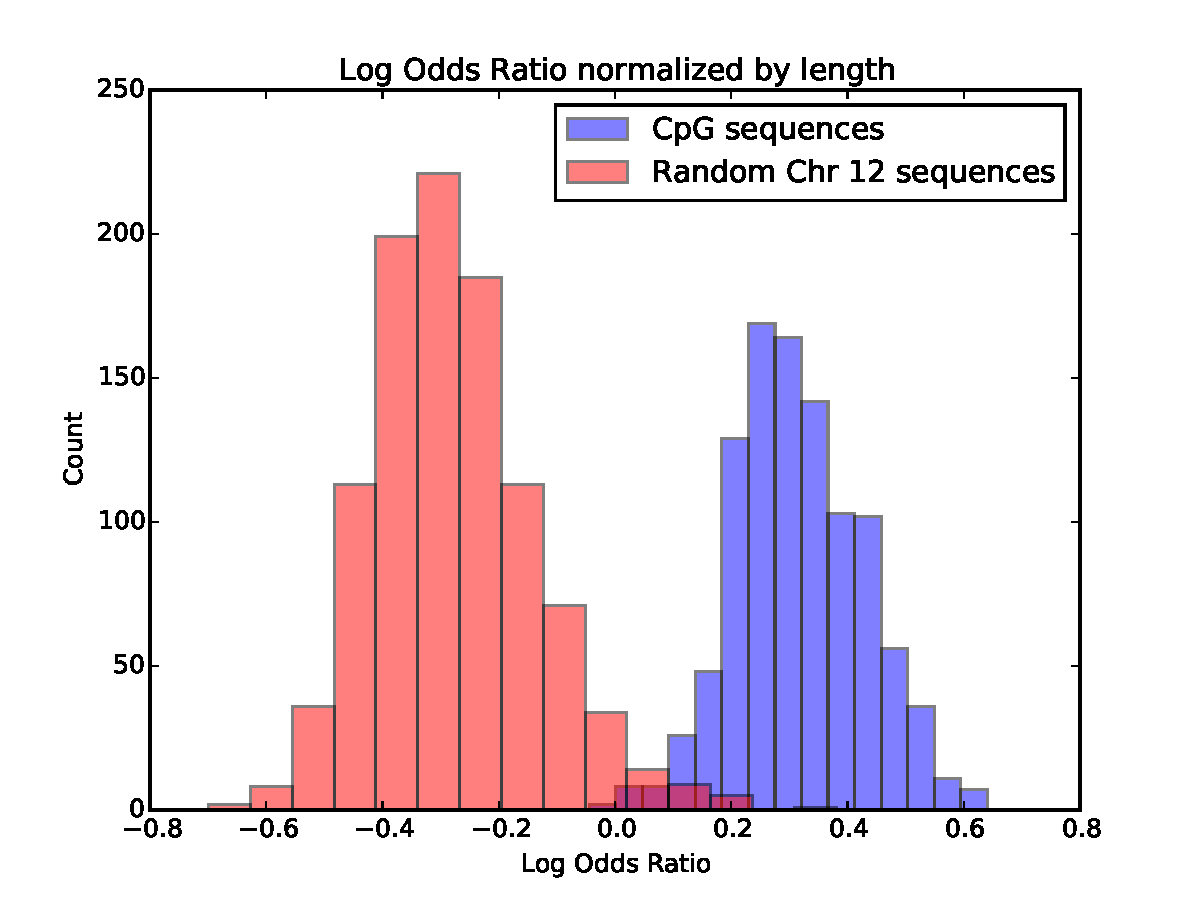
\includegraphics[trim={0 0 2cm 0}, clip,width=3.5in]{histogram.pdf}
%	\caption{Histogram of log odds ratios of the positive and negative test sets normalized for the length of the sequences}
%	\label{fig:hist}
%\end{figure}



%
% The following two commands are all you need in the
% initial runs of your .tex file to
% produce the bibliography for the citations in your paper.
\bibliographystyle{abbrv}
%\bibliography{sigproc}  % sigproc.bib is the name of the Bibliography in this case

% You must have a proper ".bib" file
%  and remember to run:
% latex bibtex latex latex
% to resolve all references
%
% ACM needs 'a single self-contained file'!
%
%APPENDICES are optional
%\balancecolumns

\balancecolumns
% That's all folks!
\end{document}
